Suppose $N\ge 1$ is an integer and define $h = 1/(N+1)$ 
and $x_k = kh$ for $k = 0, \ldots, N+1$.
Consider the $N$ \emph{hat functions}, defined as\\[0em]

\[ \hspace*{-20em}\phi_k(x) = \left\{ \begin{array}{ll}
           (x-x_{k-1})/h, & x\in [x_{k-1}, x_k);\\
           (x_{k+1}-x)/h, & x\in [x_k, x_{k+1});\\
            0,             & \mbox{otherwise}.
          \end{array}\right. \]

\vspace*{-7em}
\hspace*{25em}
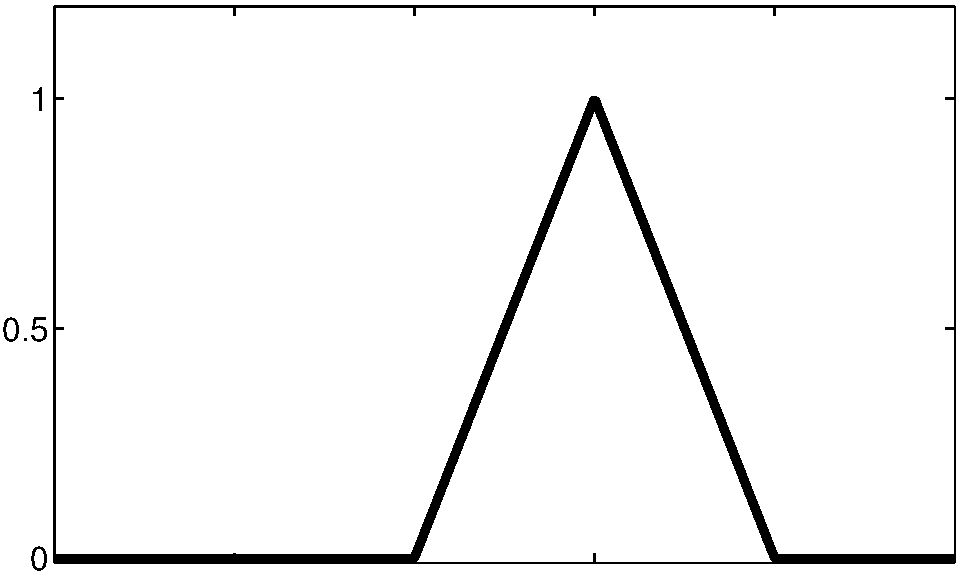
\includegraphics[scale=0.35]{hats}
\begin{picture}(0,0)
\put(-159,-4){\footnotesize $x_0$}
\put(-129,-4){\footnotesize $x_1$}
\put(-99,-4){\footnotesize $x_2$}
\put(-69,-4){\footnotesize $x_3$}
\put(-39,-4){\footnotesize $x_4$}
\put(-9,-4){\footnotesize $x_5$}
\put(-50,50){\footnotesize $\phi_3(x)$}
\end{picture}

\vspace*{-1.5em}
The plot to the right shows $\phi_3(x)$ for $N=4$.

Consider the standard inner product on $C[0,1]$,
\[ (u,v) = \int_0^1 u(x) v(x)\, dx.\]

\begin{enumerate}
\item Compute the inner products $(\phi_j, \phi_k)$ for $k=1,\ldots, N$,\\
obtaining answers that depend on $N$ (or $h$) only.
Consider the following cases individually:
\begin{itemize}
\item $(\phi_j, \phi_j)$ for $j=1,\ldots, N$;
\item $(\phi_j, \phi_{j+1})$ for $j=1, \ldots, N-1$;
\item $(\phi_j, \phi_k)$ for $|j-k| > 1$.
\end{itemize}

% \vspace*{1em}\hfill \emph{problem continues on the next page}
%
% \newpage
\item For $f(x) = \sin(\pi x)$, 
      compute the inner products $(\phi_k, f)$ for $k=1,\ldots, N$.


\item Use your solutions to~(a) and~(b) to set up a linear system (in MATLAB)
      and solve it to compute the best 
      approximations $f_N(x)$ from ${\rm span}\{\phi_1, \ldots, \phi_N\}$ to 
      $f(x) = \sin(\pi x)$ for $N=3$ and $N=9$ over the interval $[0,1]$
      with the standard inner product.  

      For each of these $N$, use the \verb|hat.m| code (from Problem Set~1, 
      either your code or from the solutions) to plot your best approximations.
      For each $N$, produce one plot that compares $f_N(x)$ to $f(x)$,
      and a second plot that shows the error $f(x) - f_N(x)$.

      [Be careful: Are the basis functions used for the best approximation orthogonal?]
\end{enumerate}

%%%%%%%%%%%%%%%%%%%%%%%%%%%%%%%%%%%%%%%%%%%%%%%%%%%%%%%%%%%%%%%%%%%%%%%%%%%%%%%%

\ifthenelse{\boolean{showsols}}{\begin{solution}
\begin{enumerate}
\item To find $\ip{\phi_j, \phi_k}$, we integrate only over the \emph{support}
      of the integrand, that is, we only consider the region of $[0,1]$ on which
      $\phi_j(x)\phi_k(x)$ is nonzero.
     \begin{itemize}
     \item First we consider $j=k$.  Note that the answer (the area under the square
           of a hat function) is independent of placement on the $x$ axis,
           so we can pick the interval of integration as convenient:
          \begin{eqnarray*}
           \ip{\phi_j, \phi_j} &=& \int_{x_{j-1}}^{x_j} \Big({x-x_{j-1} \over h}\Big)^2\, dx 
                                 + \int_{x_j}^{x_{j+1}} \Big({x_{j+1}-x \over h}\Big)^2\, dx 
                                 \\[0.5em]
                               &=& \int_0^h {x^2 \over h^2} \, dx 
                                 + \int_{-h}^0 {(-x)^2 \over h^2}\, dx \\[0.5em]
                               &=& {h^3 \over 3h^2} + {h^3 \over 3h^2}  = {2h\over 3}.
         \end{eqnarray*}
     \item Next we consider the inner product of two adjacent hat functions, 
           $\ip{\phi_j,\phi_{j+1}}$, noting that the support of the two functions
           $\phi_j$ and $\phi_{j+1}$ only overlaps on $(x_j, x_{j+1})$.
           Again shifting to integration to a convenient region, we have:
          \begin{eqnarray*}
           \ip{\phi_j, \phi_{j+1}} 
                   &=& \int_{x_j}^{x_{j+1}} \Big({x_{j+1}-x \over h}\Big)
                                            \Big({x-x_j \over h}\Big)\, dx \\[0.5em]
                               &=& \int_0^h \Big({h-x \over h}\Big)
                                            \Big({x \over h}\Big) \, dx  \\[0.5em]
                               &=& {h^3 \over 2h^2} - {h^3 \over 3h^2}  = {h\over 6}.
         \end{eqnarray*}
     \item Finally, we note that $\ip{\phi_j, \phi_k} = 0$ when $|j-k|>1$,
           as the supports of $\phi_j$ and $\phi_k$ do not overlap and hence
           $\phi_j(x)\phi_k(x) = 0$ for all $x\in[0,1]$.
     \end{itemize}
\item The inner products $\ip{\phi_j, \sin(\pi x)}$ are tedious to compute by hand;
      one requires one integration by parts and a considerable amount of tedious algebra
      to arrive at the formula
          \begin{eqnarray*}
              \ip{\phi_j, f} &=& \int_{x_{j-1}}^{x_j} {x-x_{j-1} \over h} \sin(\pi x)\, dx
                              + \int_{x_j}^{x_{j+1}} {x_{j+1}-x \over h} \sin(\pi x)\, dx \\[0.5em]
                             &=& {2 \sin(\pi x_j) - \sin(\pi x_{j-1}) - \sin(\pi x_{j+1}) 
                                   \over \pi^2 h} \\[0.5em]
                             &=& {2\sin(\pi x_j) \over \pi^2 h} (1 - \cos(h\pi)).
         \end{eqnarray*} 

\item The requested plots are shown below, followed by the MATLAB code that generated them.

\vspace*{1em}
{[\textbf{GRADERS:} Please deduct 10~points for solutions that treat the hat functions as if they are
orthogonal, and thus don't set up a Gram matrix to determine the coefficients of the best
approximation.]}

\begin{center}
   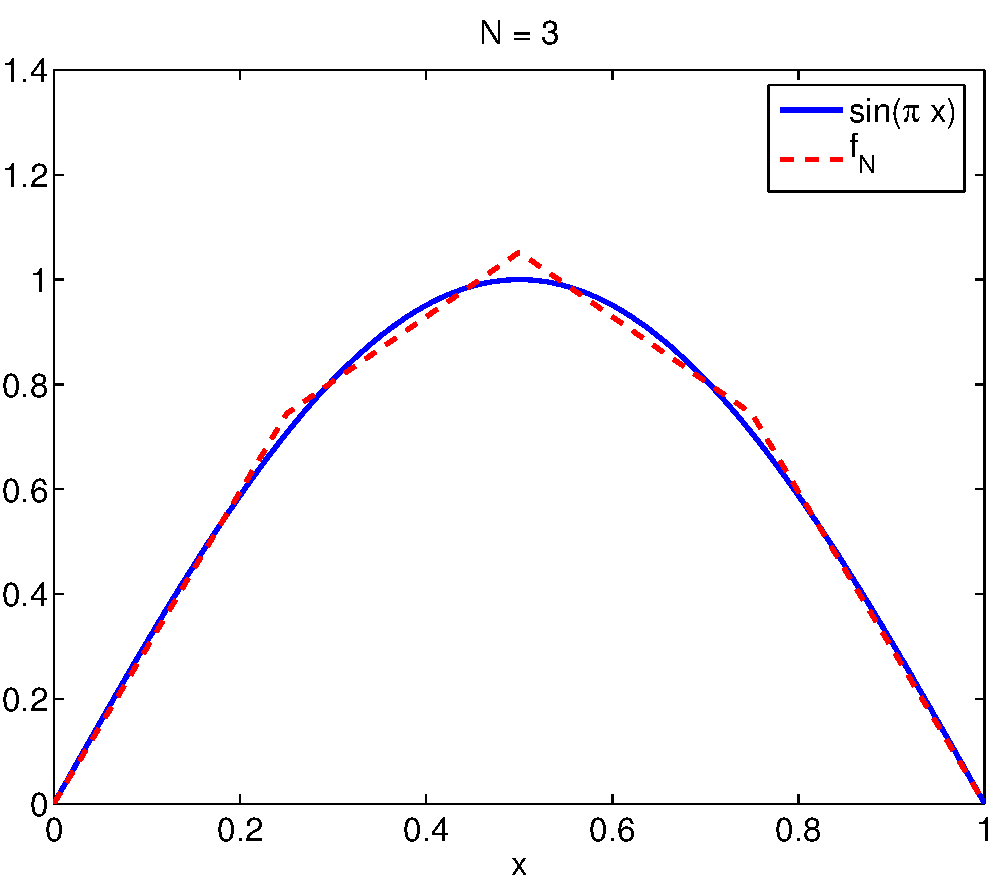
\includegraphics[scale=0.4]{hats_3a}\quad 
   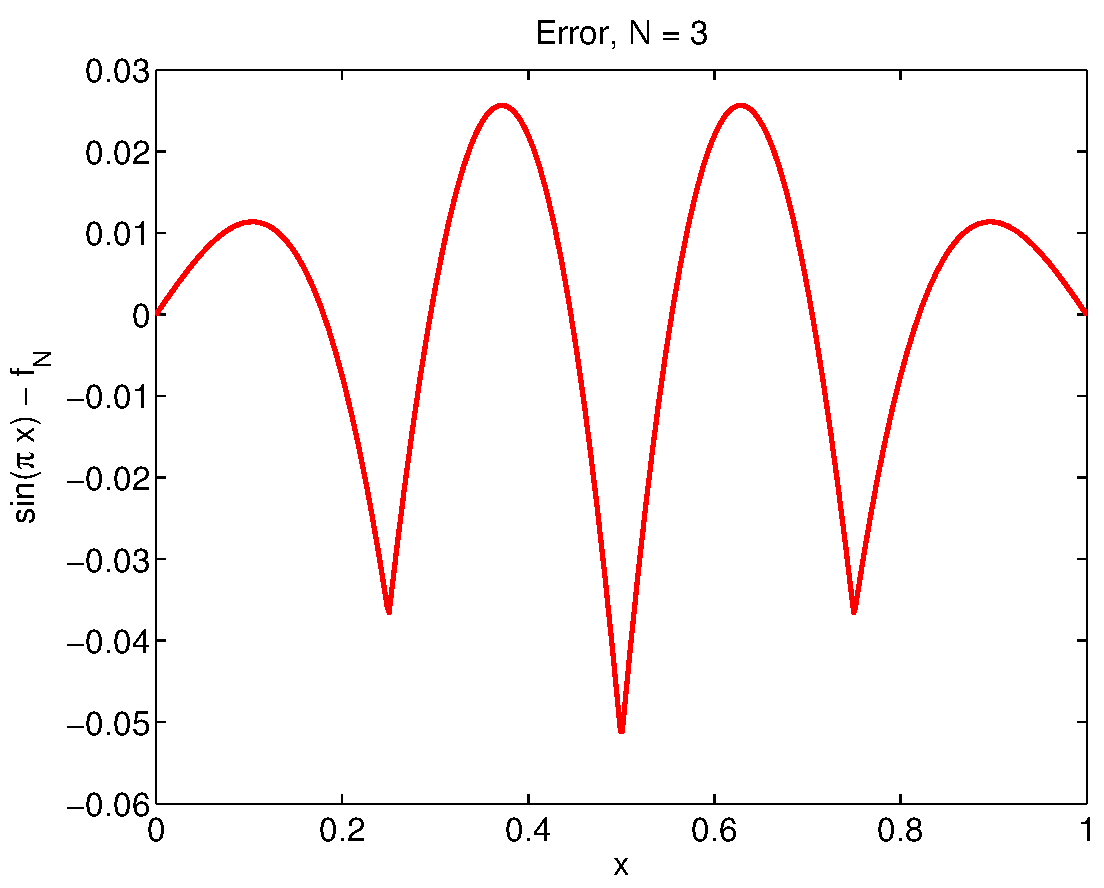
\includegraphics[scale=0.4]{hats_3b}

   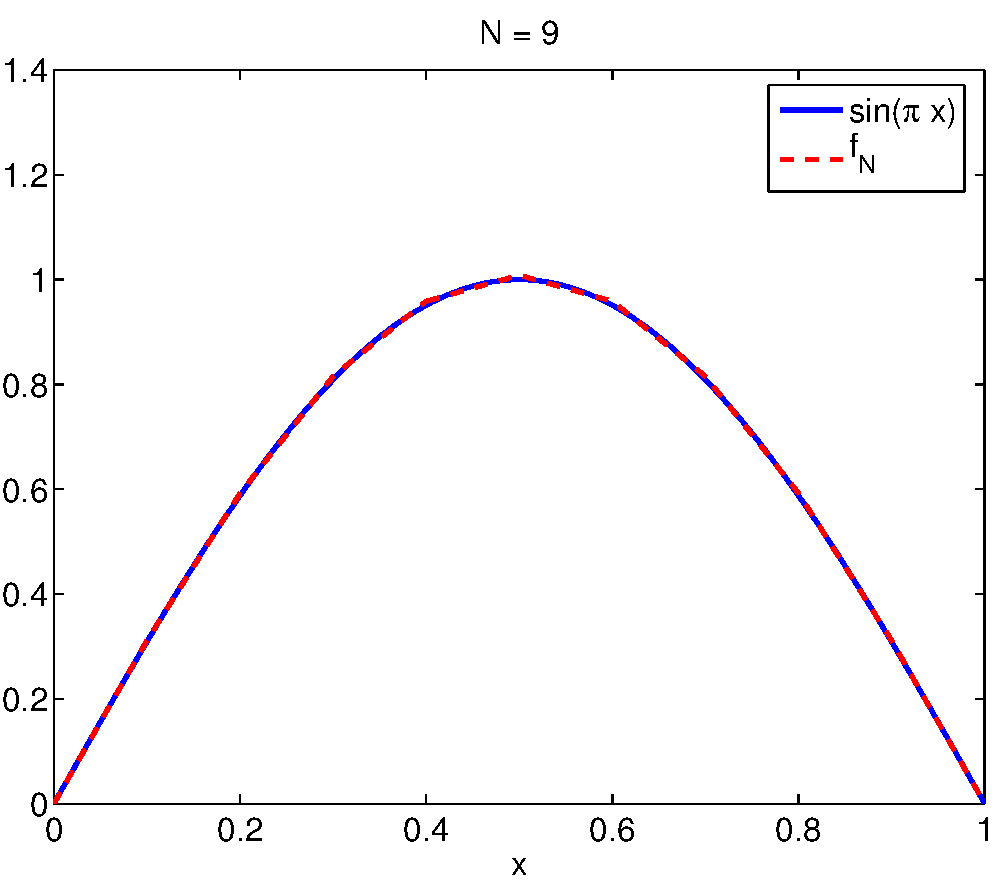
\includegraphics[scale=0.4]{hats_9a}\quad 
   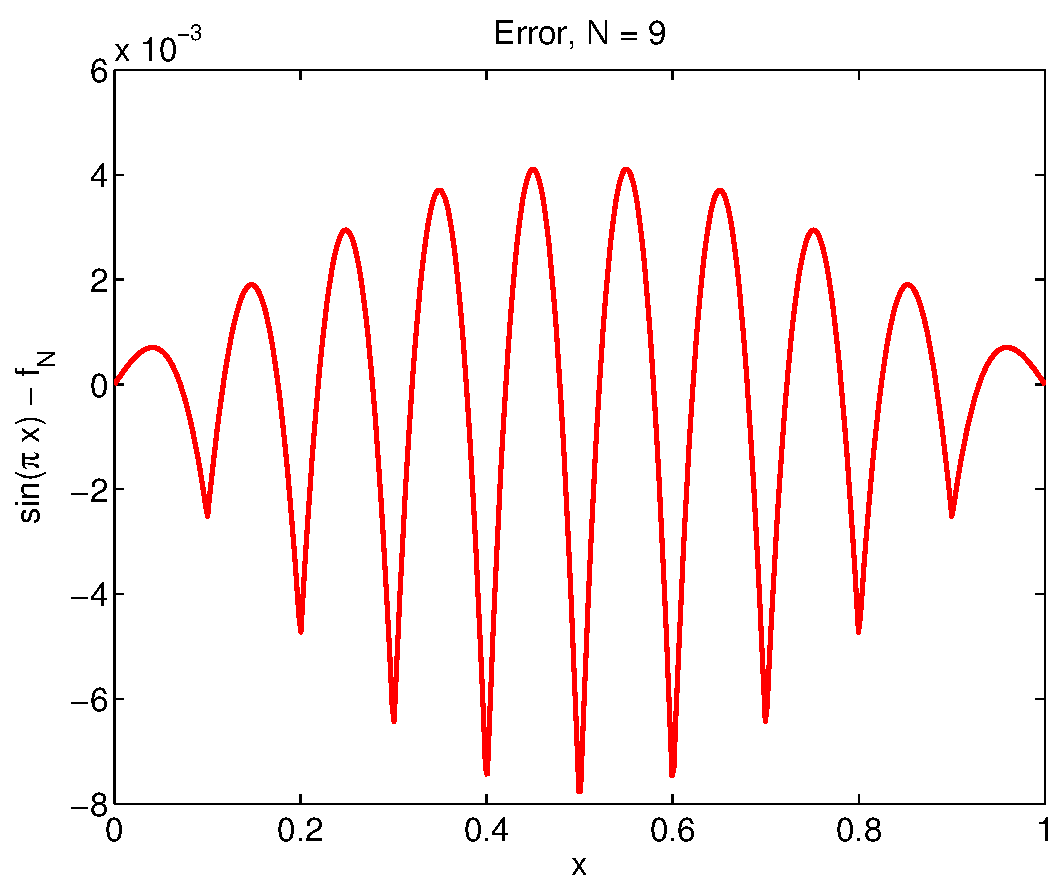
\includegraphics[scale=0.4]{hats_9b}
\end{center}

\input hats_code
\end{enumerate}
\end{solution}}{}

